\documentclass[5pt]{article}
\title{\LARGE {Note for vortex phase transition in iron-based superconductor}}
\author{\Large{Wei Cheng}}
\date{\Large{2023.3.17}}
\usepackage{amsmath,amsthm,amssymb,amsfonts, fancyhdr, color, comment, graphicx, environ}
\usepackage{verbatim}
\usepackage[UTF8]{ctex}%用于识别中文
\usepackage{underscore}%可以用来正确识别_
\usepackage{graphicx}%用于插入图片
\usepackage{geometry}
\usepackage{braket}
\usepackage{listing}
\geometry{a4paper,scale=0.85}
\usepackage{hyperref}%用于插入链接
\hypersetup{
	colorlinks=true,
	linkcolor=blue,
	filecolor=magenta,      
	urlcolor=blue,
}%插入链接的性质
\usepackage{pythontex}
\usepackage{import}
\usepackage{subfiles}
\usepackage{xifthen}
\usepackage{pdfpages}
\usepackage{transparent}
\usepackage{framed}
\usepackage{tcolorbox}
\usepackage[dvipsnames,svgnames]{xcolor}
\usepackage{abstract}
\usepackage{pgfplots,tikz}
\tcbuselibrary{skins,breakable,xparse}
\usepackage{shadowtext}
\usepackage{titlesec}
\usepackage{titletoc}
\usepackage{setspace}
\usepackage{float}
\usepackage{enumitem}  
\usepackage[normalem]{ulem}
\usepackage[charter]{mathdesign}
\usepackage{shadowtext}
\usepackage{setspace}
\usepackage{tabularcalc}
\usepackage{booktabs}
\usepackage[citecolor=red]{hyperref}%用于插入链接
\hypersetup{
	colorlinks=true,
	linkcolor=blue,
	filecolor=red,      
	urlcolor=blue,
	citecolor=red
}%插入链接的性质
\usepackage{ragged2e}




\renewcommand{\abstractname}{\Large Abstract}
\renewcommand\refname{\LARGE Reference}




\definecolor{mygreen}{rgb}{0.8,1,0.73}
\definecolor{linegreencolor}{rgb}{0,0.4,0}
\definecolor{myblue}{rgb}{0.22,0.73,0.91}
\definecolor{LightBlue1}{rgb}{0.22,0.73,0.91}
\definecolor{myteal}{cmyk}{0.5,0,0.15,0}
\definecolor{myred}{RGB}{255,182,185}
\definecolor{myredline}{RGB}{228,44,100}

\titleformat*{\section}{\Large\bfseries\filcenter}
\titleformat*{\subsection}{\Large\bfseries}
\titleformat*{\subsubsection}{\Large\bfseries}
\titleformat*{\paragraph}{\large\bfseries}
\titleformat*{\subparagraph}{\large\bfseries}

\renewcommand*\contentsname{\hfill \LARGE{Content} \hfill}

\newcommand{\upcite}[1]{\textsuperscript{\textsuperscript{\cite{#1}}}}
\begin{document}
	\maketitle
	\Large
	\tableofcontents
	\everymath{\displaystyle}
	\begin{abstract}
		\Large
		Iron-based superconductor is a very good platform to search Majorana zero model due to it's topological band and high temperature superconductor.Here we search the vortex phase transition in iron-based superconductor.First we can use the $k\cdot p$ method to construct the Hamiliton.Then use the Hamiliton we can do some numerical calculation and theory analysis.
	\end{abstract}
\section{$k\cdot p$ construct Hamiliton}
The space group of iron-based superconductor is P4/nmm,it include the frational translate,so it can't can be seen the the direct product of the translate group and the point group.But along the $\Gamma-Z$,it can be seen the $D4h$ group。At the same time,we can know the band near the fermi surface of the iron-based superconductor are $p_z,d_{xz},d_{yz}$ orbit.So we can choose the basics $\ket{p_z,\uparrow},\ket{p_z,\downarrow},\ket{d_{xz+iyz},\downarrow},\\
\ket{d_{xz-iyz},\uparrow},\ket{d_{xz+iyz},\uparrow},\ket{d_{xz-iyz},\downarrow}$ to construct our Hamiliton.
The structure of the iron-based superconductor and the band structure as follows.
\begin{figure}[H]
	\centering
	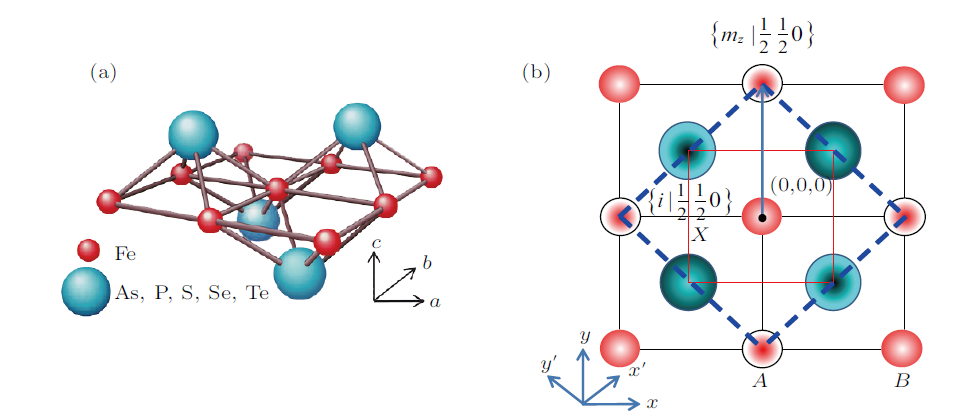
\includegraphics[scale=0.8]{figure/3}
	\caption{\cite{胡江平铁基}}
	\label{}
\end{figure}

\begin{figure}[ht]
	\centering
	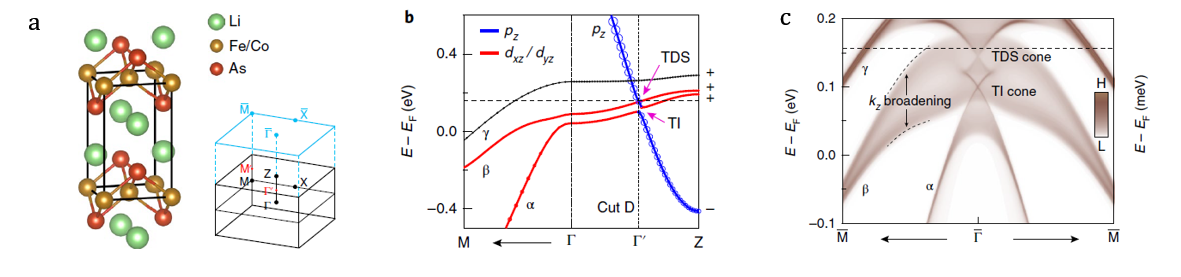
\includegraphics[scale=0.6]{figure/4}
	\caption{\cite{zhang2019multiple}}
	\label{}
\end{figure}


For any $6\cdot 6$matrix,we can break down to the linear superposition of 36 basics matrix.
\begin{align}
	H(\vec{k})=\sum_{ij}f_{ij}(\vec{k})M_{ij}
\end{align}
we can construct the 36 basics Hermitian matrix from the direct product of the Pauli matrix and the Gellman matrix.
\begin{align}
	M_{ij}=G_i\otimes \sigma_j
\end{align}
The $G_i$ means the Gell-Man matrix,it's range is from 0 to 8.The $\sigma_j$ means the Pauli matrix,it's range is from 0 to 3. 
At the same time,because we need to consider the spin orbit coupling,so we neend sonsider the double group,we can find the character table of the D4h.
\begin{figure}[H]
	\centering
	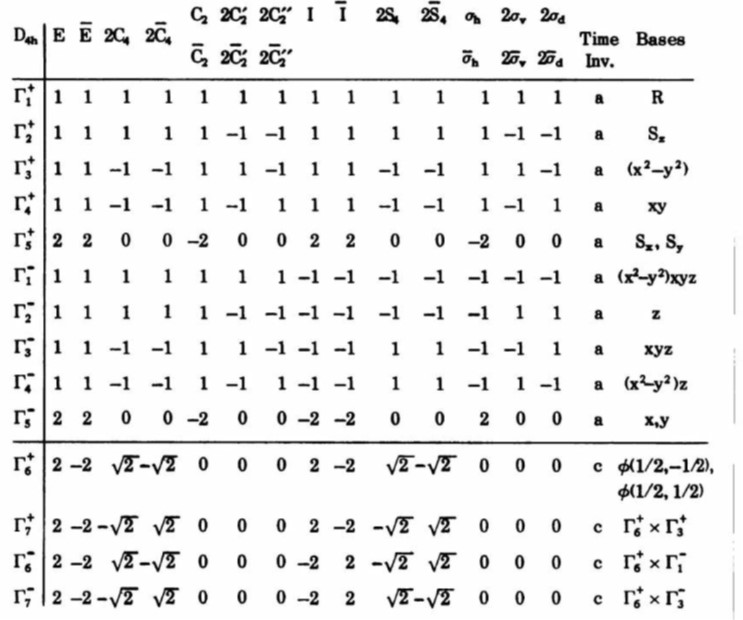
\includegraphics[scale=0.8]{figure/1}
	\caption{}
	\label{}
\end{figure}
We can get the generator of D4h group is $C_{4z},C_{2x}^{'},Inversion$.At the same time,the system has the time reversal symmetry.We can get the transformation matrix in the basics before we mentioned.So we can get the Hamiliton for the iron-based superconductor.
\begin{align}
	\nonumber
	H&=M_1(k)M_{30}+M_2(k)M_{80}+A_1k_xM_{21}+A_1k_yM_{22}+A_2k_xM_{50}+A_2k_yM_{43}
	\\
	\nonumber  &\qquad +B_1k_zM_{23}+C_1k_xk_zM_{63}-C_1k_yk_zM_{70}+D_1(k_x^2-k_y^2)M_{61}+D_2k_xk_yM_{62}
\end{align}

\begin{normalsize}
\begin{align}
	C_{4z}=
	\frac{1}{\sqrt{2}}
	\begin{pmatrix}
		1-i&&&&&\\
		&1+i&&&&\\
		&&1-i&&&\\
		&&&1+i&&\\
		&&&&-1-i&\\
		&&&&&-1+i
	\end{pmatrix}
\qquad
C_{2x}=\begin{pmatrix}
	&i&&&&\\
	i&&&&&\\
	&&&i&&\\
	&&i&&&\\
	&&&&&i\\
	&&&&i&
\end{pmatrix}
\end{align}
\begin{align}
	I=\begin{pmatrix}
		-1&&&&&\\
		&-1&&&&\\
		&&1&&&\\
		&&&1&&\\
		&&&&1&\\
		&&&&&1
	\end{pmatrix}
\qquad
T=
\begin{pmatrix}
&-1&&&&\\
1&&&&&\\
&&&-1&&\\
&&1&&&\\
&&&&&-1\\
&&&&1&\\	
\end{pmatrix}
\mathcal{K}
\end{align}
\end{normalsize}
we can get the character table of the polynomials
of the momentum k
\begin{align}
	\nonumber
	\begin{tabular}{ccc}
		\toprule
		\midrule
		k polynomial & representation & time reversal \\
		1,$k_x^2+k_y^2$,$k_z^2$ &$\Gamma_1^{+}$&+\\
		$k_xk_y$&$\Gamma_4^{+}$&+\\
		$k_x^2-k_y^2$&$\Gamma_3^{+}$&+\\
		$\{k_xk_z,k_yk_z\}$&$\Gamma_5^{+}$&+\\
		$\{k_x,k_y\}$&$\Gamma_5^{-}$&-\\
		$k_z$&$\Gamma_2^{-}$&-
	\end{tabular}
\end{align}
we can get the character table of $M_{ij}$,Then we can multiple the same representation of the k polynomials and the $M_{ij}$ matrix.So we can get the Hamiliton of the iron-based superconductor.
\begin{align}
	\nonumber
	H&=M_1(k)M_{30}+M_2(k)M_{80}+A_1k_xM_{21}+A_1k_yM_{22}+A_2k_xM_{50}+A_2k_yM_{43}
	\\
	\nonumber  &\qquad +B_1k_zM_{23}+C_1k_xk_zM_{63}-C_1k_yk_zM_{70}+D_1(k_x^2-k_y^2)M_{61}+D_2k_xk_yM_{62}\\
	&=	\begin{pmatrix}
		M_1(k)      &     0        &   -iB_1k_z        &   -iA_1k_{-}     &   -iA_2k_{+}    &0\\
		0  &     M_1(k)      &  -iA_1k_{+}    &   iB_1k_z       &     0     & -iA_2k_{-}\\
		iB_1k_z    &   iA_1k_{-}      &    -M_1(k)        & 0     &   C_1kzk_{+} &D(k_x,k_y)\\
		iA_1k_{+}    &   -iB_1k_z    &   0  &   -M_1(k)    & D(k_x,k_y)^{*} &C_1k_zk_{-}\\
		iA_2k_{-}  &        0    &    C_1k_zk_{-}    &    D(k_x,k_y)      &      -M_1(k)+\delta_{so}      &0\\
		0&      iA_2k_{+}      &   D(k_x,k_y)^{*}    &   C_1k_zk_{+}       &    0      & -M_1(k)+\delta_{so} \\
	\end{pmatrix}
\end{align}	
\begin{figure}[H]
	\centering
	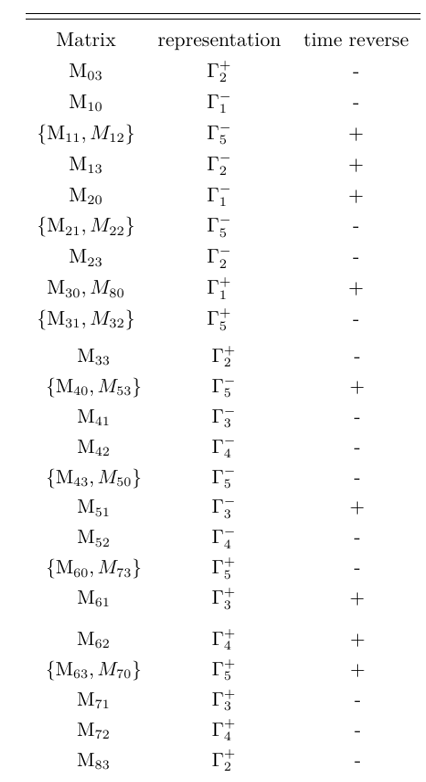
\includegraphics[scale=0.8]{figure/2}
	\caption{}
	\label{}
\end{figure}




\section{Vortex Phase Transition}
As we were know,when the $\delta_{so}$ is very big,the three band can be seen the independent of the TI and DSM.At this time,the topological vortex phase transition(VPT) can be seen the independent of TI and DSM use the Berry phase crition by Vishwanath.\cite{PhysRevLett.107.097001}.But when the $\delta_{so}$ become very small,the situation become complex.we need to consider the interplay of the three band.At the same time,we can consider symmetry breaking effect to it's topological properties.
\par 
From the $k\cdot p$ method,we can get the Hamiliton of the iron-based superconductor.So we can do some mumerical calculation and the theory analysis.When we breaking $C_{4z}$ symmetry to $C_{2z}$,the symmetry group will from $D_{4h}$ down to $D_{2h}$,with the same analysis,we can know that it's Hamiliton will add $A_{z}^{'}M_{41}$,it will open the gap of the DSM.Then we can consider the vortex along the x directation,and calculate it's Energy at $k_x=0$ change by $\mu$.We can find somethings from the numerical result.First,when $A_z^{'}>0$,the VPT's eigvalue of the $C_{2x}=-1$ and when the $\delta_{so}$ is decrease,the VPT point from 4 change to 1.Second,when change the sign of the $A_{z}^{'}$,one part of the VPT's eigvalues of the $C_{2x}$ change from -1 to +1.we can understand this phenon from the theory analysis when the $\delta_{so}\rightarrow \infty$ and $\delta_{so}=0$.For theory simpilipy,we consider the vortex along the z direction,and change the parameter of the $k_y$.
\par 
The vortex line is the 1D topological superconductor system,which belong to 1D D class of the Altland-Zirnbauer classification of topological phases.So we can define $Z_2$ topological invariant at $k_z=0 or \pi$ to describe it's topological properties.So we can to calculate it's gap close times to know whether it's topological or not.So the following analysis is counting the zero solution of the $H_{BdG}$ at the $k_z=0$.
\subsection{$\delta_{so}\rightarrow \infty$,change sign of $k_y$}
In this part,I want to prove that when change the sign of the parameter of $k_y$,the VPT of the TI(DSM) will change from the $C_{2z}=1(-1)$ to $C_{2z}=-1(1)$






\newpage
\bibliographystyle{IEEEtran}
\bibliography{vortex.bib}
\end{document}